\def\bm#1{\mbox{\boldmath$#1$\unboldmath}} 

\section{Evolution of theories for LHC DM searches} 
\label{sec:evolution}

The experimental results of two of the three DM search strategies, namely direct and indirect detection, are commonly interpreted in the DM effective field theory~(DM-EFT) framework. The operators in these DM-EFTs are build from SM fermions and DM fields. Schematically, one has in the case of spin-0 interactions and Dirac fermion DM
\begin{align}\label{eq:EFT}
\mathcal{L}_\text{DM-EFT}= \sum_{f=u, d, \ell} \,\left(\frac{C_{1}^f}{\Lambda^2} \bar f f \bar \chi \chi  +\frac{C_{2}^f}{\Lambda^2} \bar  f \gamma_5 f \bar \chi\gamma_5 \chi \,+\ldots \right) \,, 
\end{align}
 where the ellipsis represents additional operators not relevant for the further discussion, the sum over $f=u,d,\ell$ includes all SM quarks and leptons, the DM candidate is called $\chi$  and $\gamma_5$ denotes the fifth Dirac matrix. The above DM-EFT is fully described by the parameters
\begin{align}\label{eq:EFTparams}
\big\{ m_\chi\,,\,\, C_n^f/\Lambda^2 \big\} \,.
\end{align}
Here $m_\chi$ is the mass of the DM candidate, $\Lambda$ is the suppression scale of the higher-dimensional operators and the $C_n^f$ are the so-called Wilson coefficients. Notice that $\Lambda$ and $C_n^f$ are not independent parameters but always appear in the specific combination given in~\eqref{eq:EFTparams}. 

The DM-EFT approach is justified for the small momentum transfer $q^2\ll \Lambda^2$ in DM-nucleon scattering (set by the non-relativistic velocities of DM in the halo) and in DM annihilation (set by the mass of the annihilating DM candidate). See Figure~\ref{fig:momentumtransfer} for an illustration of the relevant scales in each experiment. Early articles~\cite{Cao:2009uw,Beltran:2010ww,Goodman:2010yf,Bai:2010hh,Goodman:2010ku,Fox:2011pm} on DM searches at colliders quantify the reach of the LHC in the parameter space in terms of~\eqref{eq:EFTparams} and similar operators. The momentum transfer at the LHC is however larger than the suppression scale,~i.e.~$q^2 \gg \Lambda^2$, for many theories of DM.  In this case, the mediator of the interaction between the dark sector and the SM can be resonantly produced and predictions  obtained using the DM-EFT framework often turn out to be inaccurate~(see for instance~\cite{Bai:2010hh,Fox:2011fx,Shoemaker:2011vi,Busoni:2013lha,Buchmueller:2013dya,Busoni:2014sya,Busoni:2014haa,Racco:2015dxa} and~\cite{Bruggisser:2016nzw,Bruggisser:2016ixa} for exceptions). 

\begin{figure}[t]
\centering
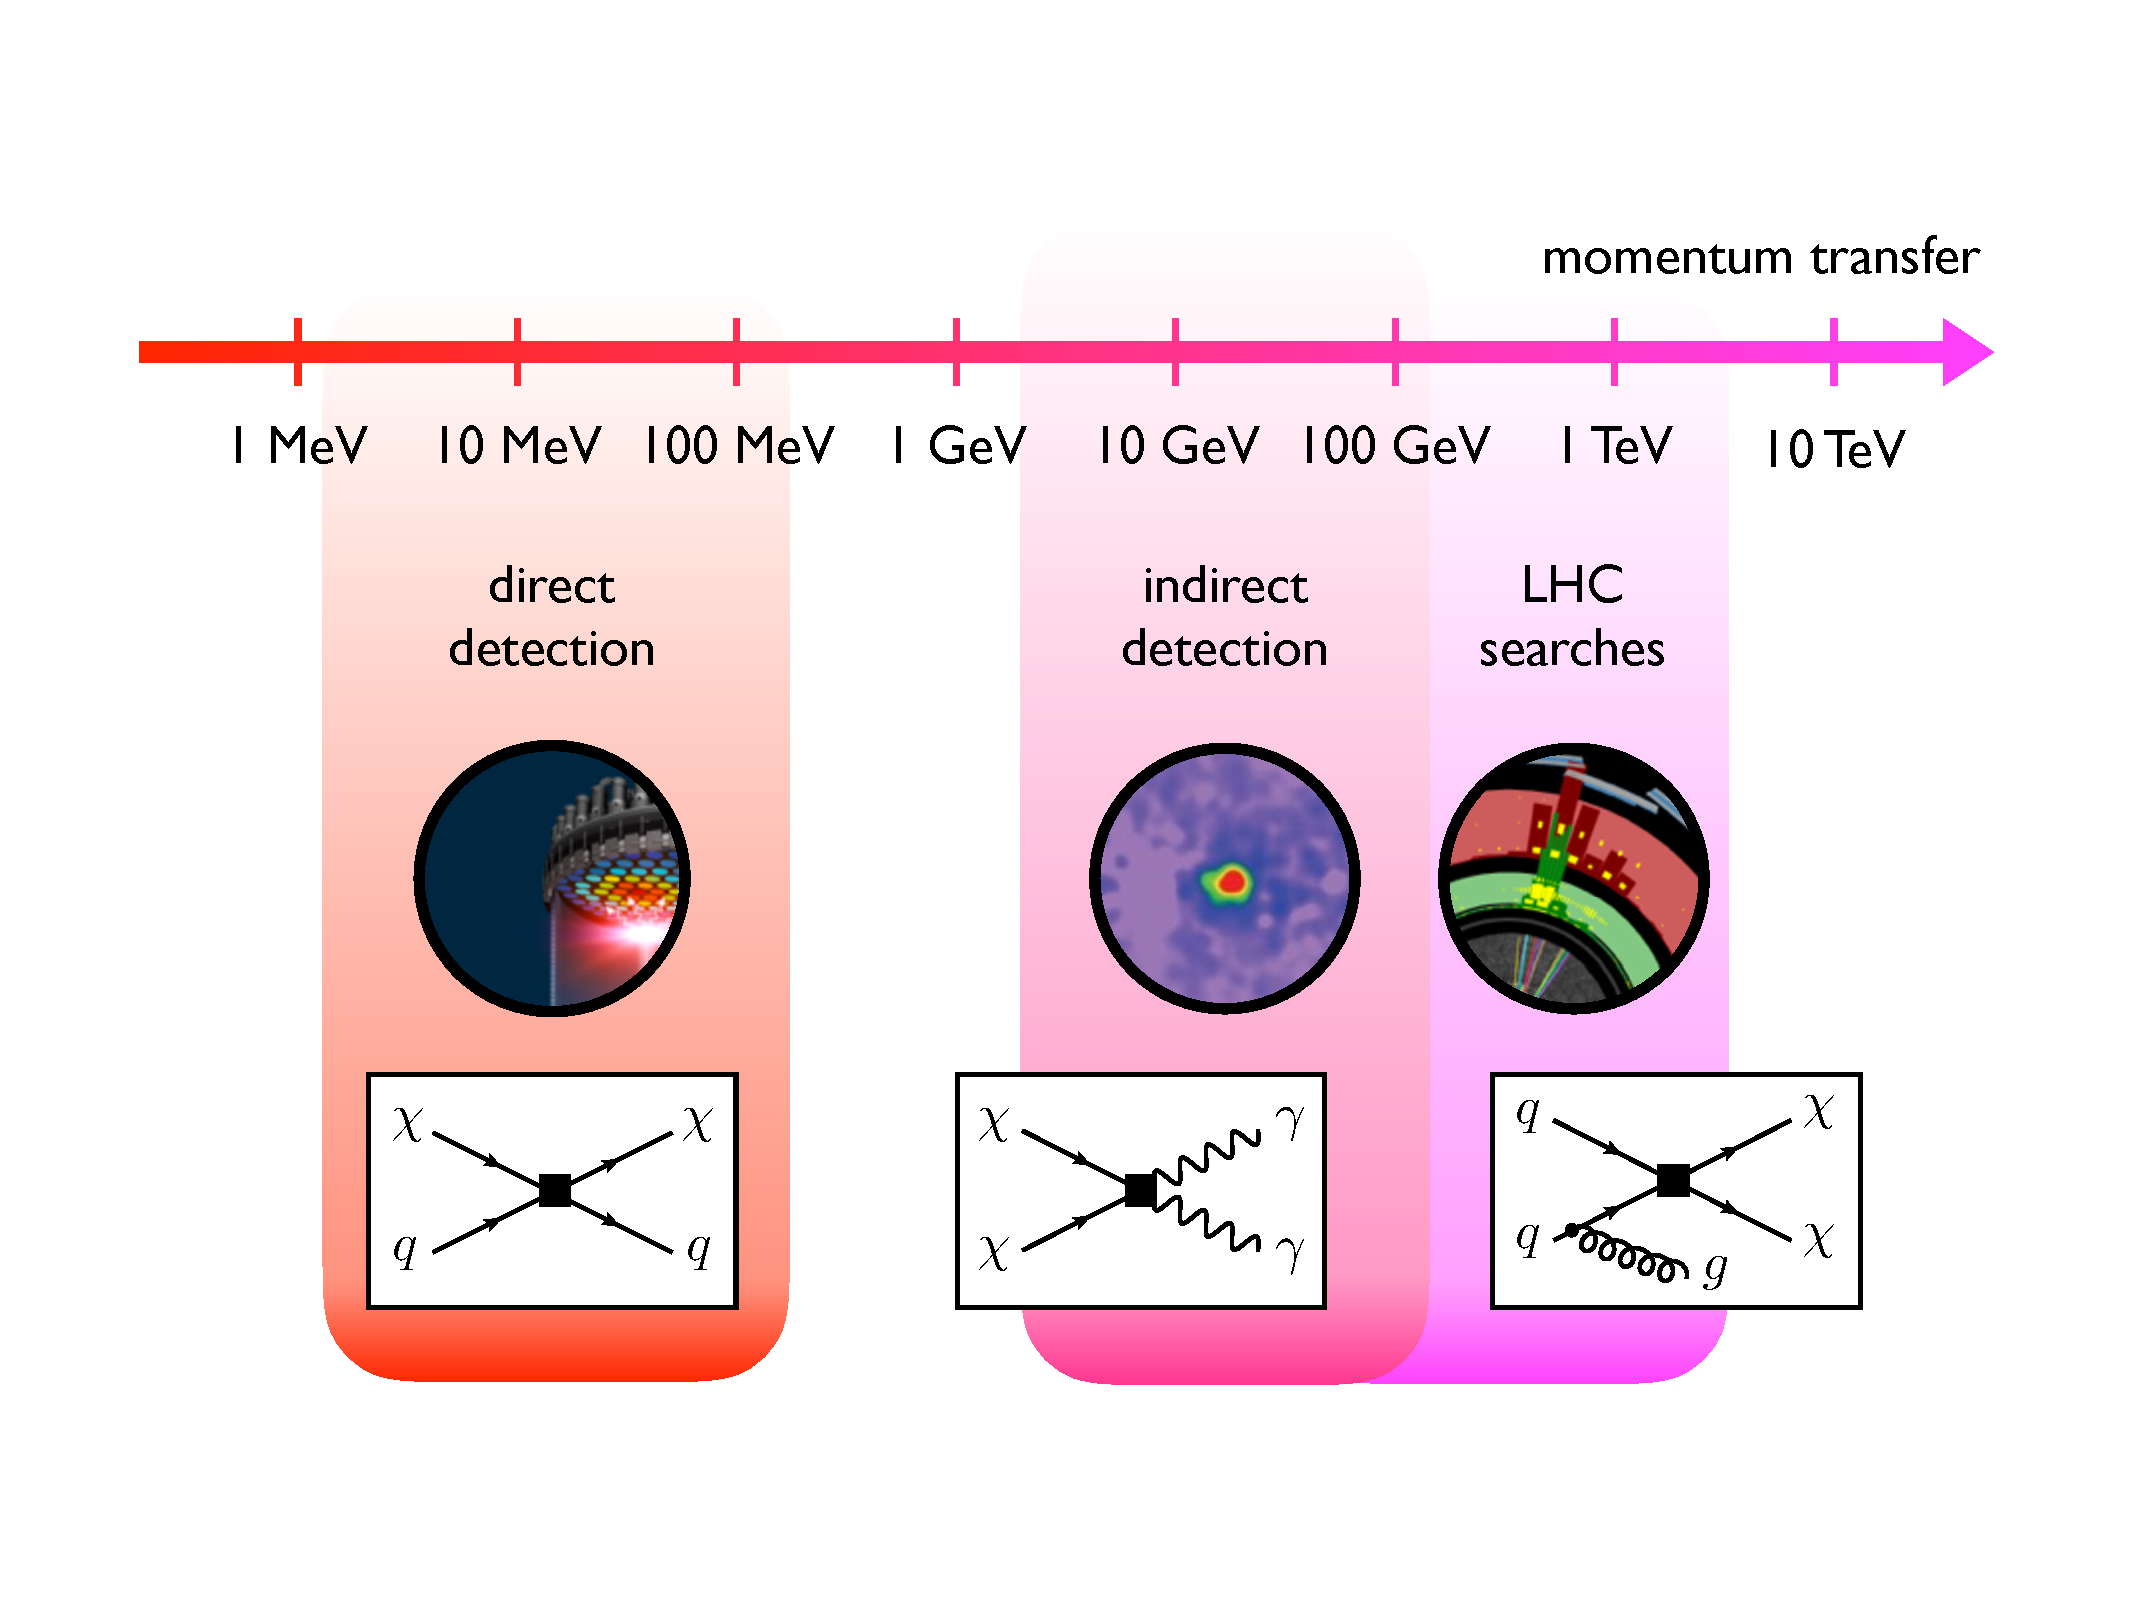
\includegraphics[width=.85\textwidth]{texinputs/00_theory/figures/figure1}
\vspace{2mm}
\caption{\label{fig:momentumtransfer} Range of momenta probed in direct-detection experiments, indirect-detection experiments and LHC searches. Prototypes of relevant Feynman diagrams are also shown. }
\end{figure}

The kinematics of on-shell propagators can be captured in DM simplified models, which aim to represent a large number of extensions of the SM, while keeping only the degrees of freedom relevant for LHC phenomenology~\cite{Abdallah:2015ter}. In the case of a pseudoscalar mediator $a$, the relevant DM-mediator and SM-mediator interactions read
\begin{align}\label{eq:simp}
\mathcal{L}_\text{DM-SIMP}=-i g_\chi a\bar \chi \gamma_5 \chi -i a \sum_j \left(g_u y_j^u \bar u_j \gamma_5 u_j + g_d y_j^d \bar d_j \gamma_5 d_j + g_\ell y_j^\ell \bar \ell_j\gamma_5 \ell_j  \right) \,,
\end{align}
with  $j$ representing a flavour index.  Since the mediator $a$ is a singlet it can also couple to itself and to $H^\dagger H$ where $H$ denotes  the SM Higgs doublet. The most general renormalisable scalar potential for a massive $a$ is therefore
\begin{align}\label{eq:VaH}
V_\text{DM-SIMP} =\frac{1}{2}m_a^2 a^2 +  b_a a^3 + \lambda_a a^4 + b_{H} a H^\dagger H +\lambda_{H} a^2H^\dagger H \,.
\end{align}
The parameters $ b_{H}$  and $\lambda_{H}$ determine the couplings between the $a$ and the $H$ fields, thereby altering both the interactions and CP properties of the SM-like scalar $h$ at $125 \, {\rm GeV}$ as well as giving rise to possible new decay channels such as $h \to aa$ (see~\cite{Curtin:2013fra,Haisch:2018kqx} for details on the LHC phenomenology). Avoiding the resulting strong constraints for any choice of~$m_a$, requires that  $b_H \ll m_a $ and $\lambda_H \ll 1$. While the former requirement can be satisfied by imposing a $Z_2$ symmetry $a \to -a$, in the latter case one has to assume that $\lambda_H$ is accidentally small if $m_a \lesssim 100 \, {\rm GeV}$ (cf.~the related discussion on invisible decays of the Higgs boson in Section~\ref{sec:constraints}). Under such an assumption and noting that the self-coupling $\lambda_a$ is largely irrelevant for collider phenomenology, the DM simplified model is  fully described by the parameters 
\begin{align}
\big\{ m_\chi, \,\, m_a\,,\,\, g_\chi\,, \,\, g_u\,,\,\,g_d\,,\,\, g_\ell \big\}\,. 
\end{align}
In fact, in the  limit of infinite mediator mass $m_a \to \infty$,  the DM-SIMP Lagrangian~\eqref{eq:simp} matches onto the DM-EFT Lagrangian~\eqref{eq:EFT}. The corresponding tree-level matching conditions are $C^f_2/\Lambda^2 = g_\chi g_f y_f  /m_a^2$ and $C_n^f=0$ for all other Wilson coefficients.

\begin{figure}
\centering
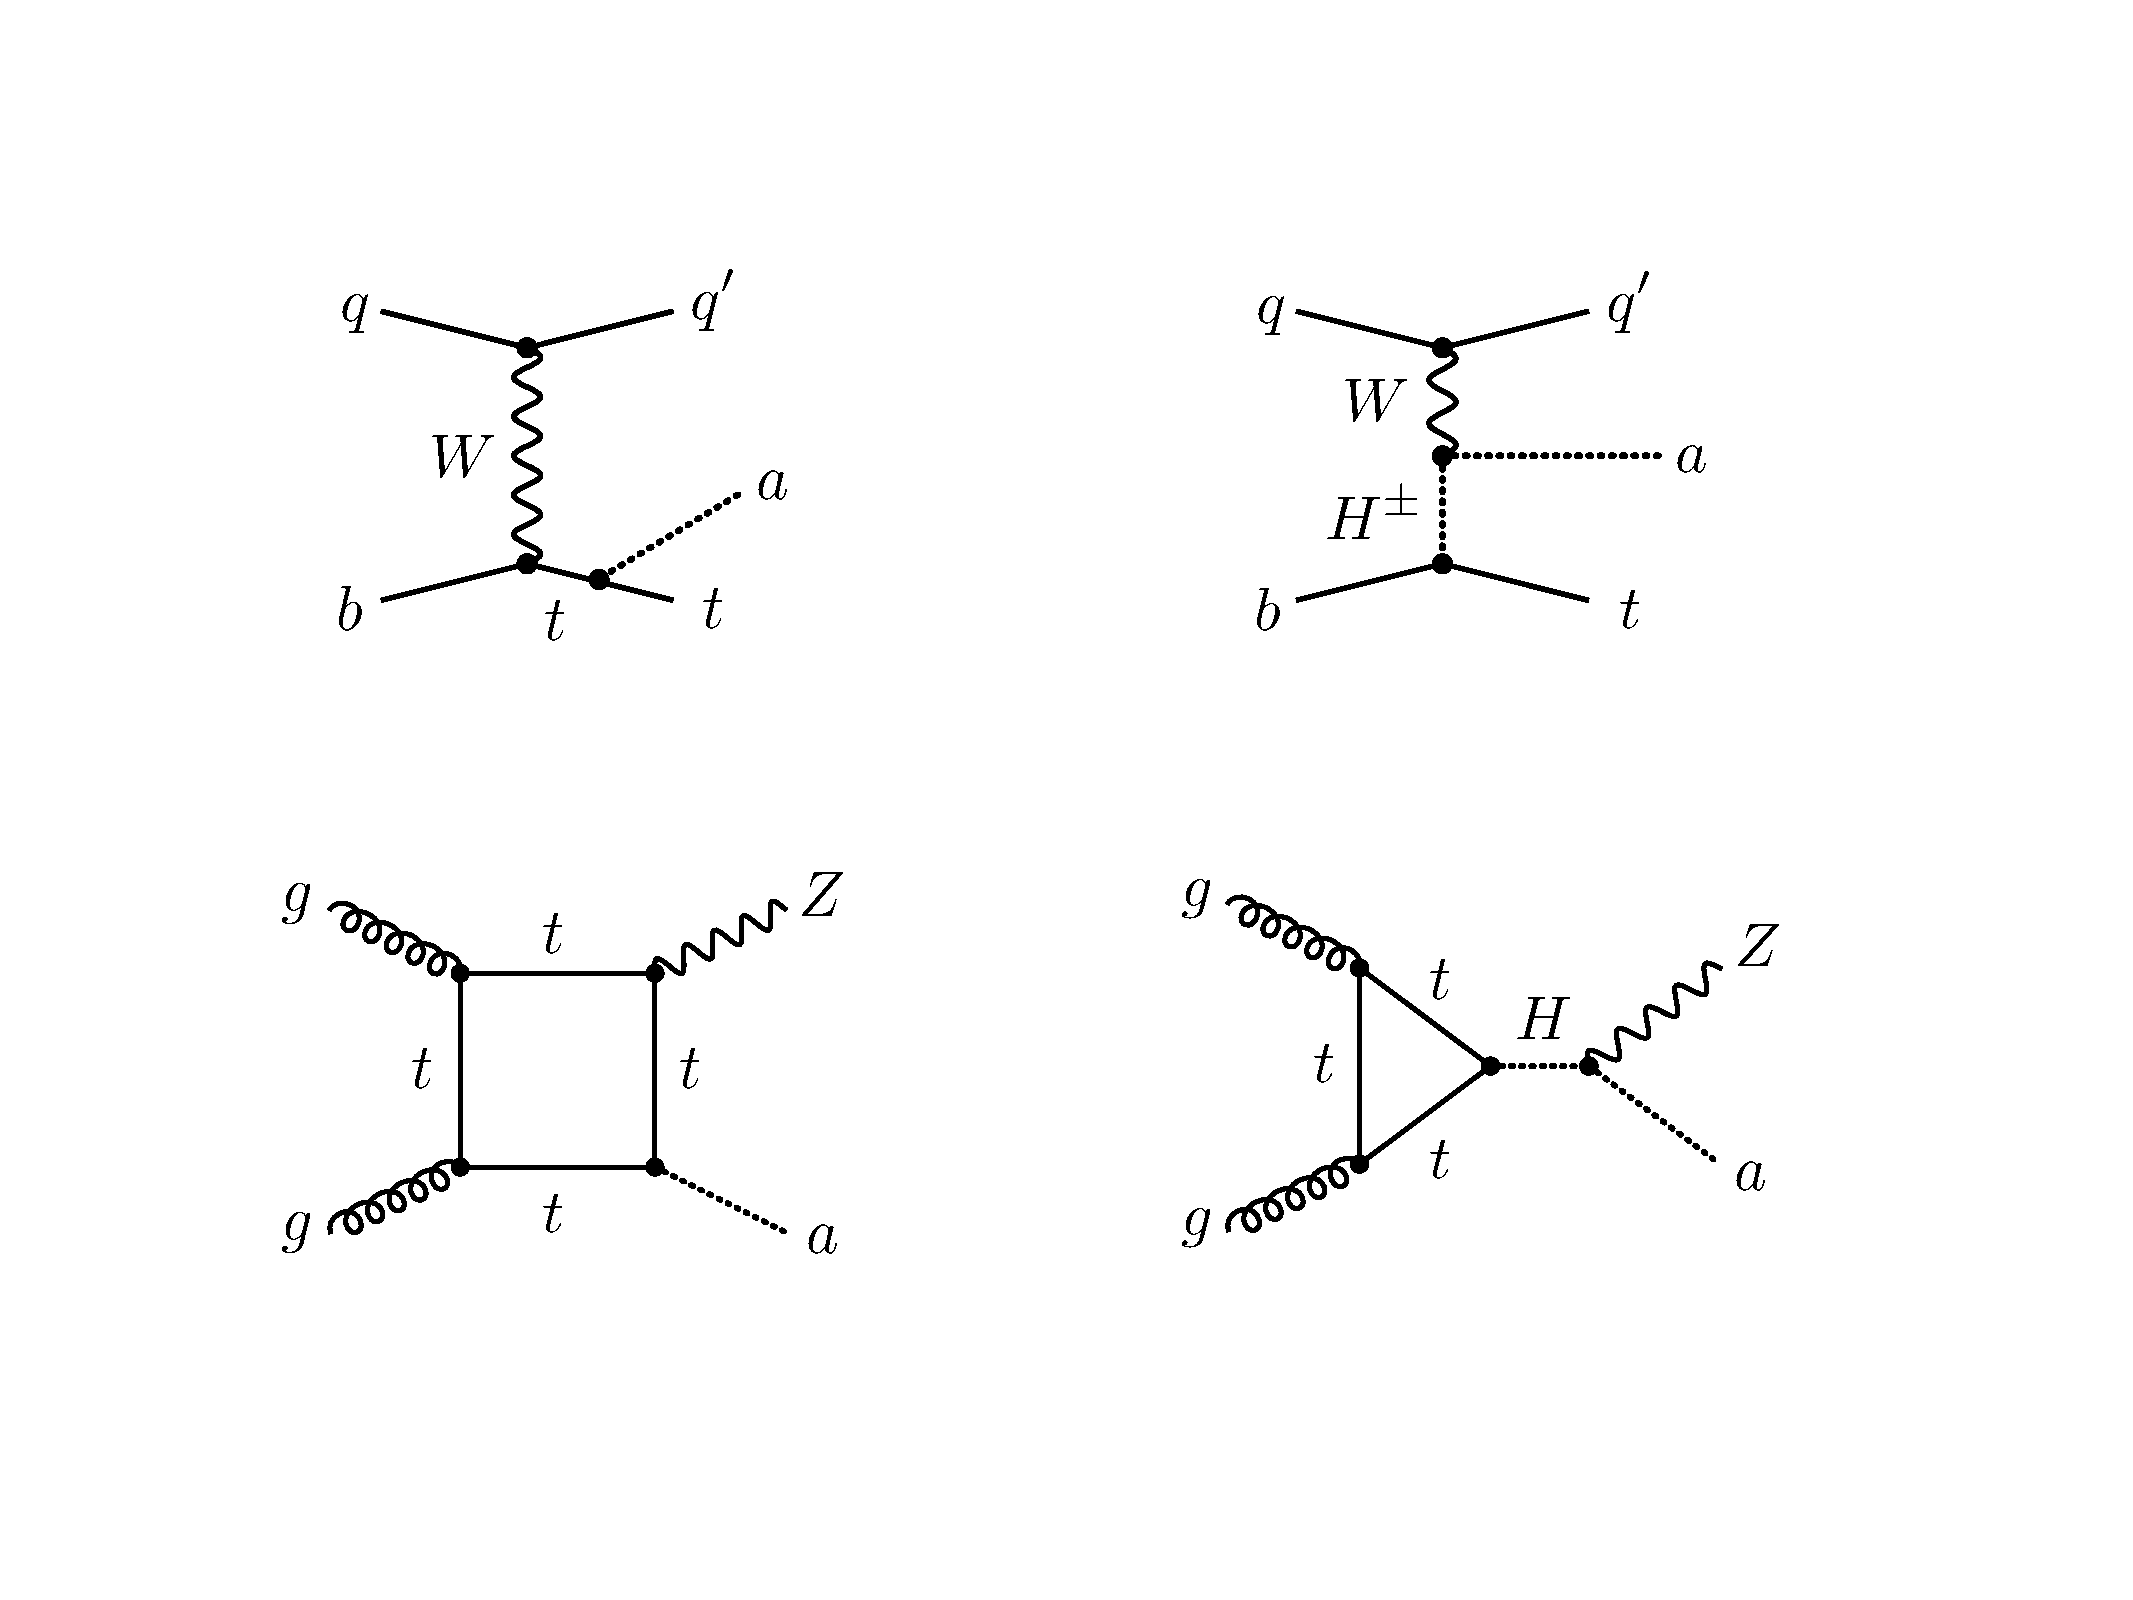
\includegraphics[width=.7\textwidth]{texinputs/00_theory/figures/figure2}
\vspace{6mm}
\caption{\label{fig:diagrams}  Diagrams contributing to the $q b \to q^\prime t a$~(upper row) and $gg \to Za$~(lower row) scattering processes.  Only the graphs on the left-hand side appear in the DM simplified model with a pseudoscalar, while in the \hdma model in addition the diagrams on the right-hand side are present. See text for further details.}
\end{figure}

Unfortunately, the operators in both $\mathcal{L}_\text{DM-EFT}$ and $\mathcal{L}_\text{DM-SIMP}$ violate gauge invariance, because the left- and right-handed SM fermions belong to different representations of the SM gauge group. In the case of the DM-EFT this suggests the Wilson coefficients~$C_n^f$ introduced in~\eqref{eq:EFT} actually scale as $C_n^f = c_n^f m_{f_i}/\Lambda$~\cite{Bell:2015sza}, whereas for the DM simplified model restoring gauge invariance requires the embedding of the mediator $a$ into an electroweak~(EW) multiplet. The absence of gauge invariance leads to unitarity-violating amplitudes in DM simplified models~(cf.~\cite{Bell:2015sza,Bell:2015rdw,Haisch:2016usn,Englert:2016joy}). In the case of the DM simplified model described by~\eqref{eq:simp}, one can show for instance that the amplitudes ${\cal A} ( q b \to q^\prime t a) \propto \sqrt{s}$ and ${\cal A} ( g g \to Z a ) \propto \ln^2 s$ diverge in the limit of large center-of-mass energy $s$. The Feynman diagrams that lead to this behaviour are depicted on the left-hand side in Figure~\ref{fig:diagrams}. Similar singularities appear in other single-top processes and in the mono-Higgs case.  Since the divergences are not power-like, weakly-coupled realisations of~\eqref{eq:simp} do not break down for the energies accessible at the LHC. The appearance of the $\sqrt{s}$ and $\ln^2 s$ terms however signals the omission of diagrams that would be present in any gauge-invariant extension that gives rise to $\mathcal{L}_\text{DM-EFT}$ in the limit where all additional particles are heavy.   For example, the $pp \to tj a$ cross section is made finite by the exchange of a charged Higgs~$H^\pm$, while in the case of $pp \to Za$  an additional scalar~$H$ unitarises the amplitude. The corresponding diagrams are displayed on the right in Figure~\ref{fig:diagrams}. Notice that the cancellation of unitarity-violating terms among the diagrams of the latter figure is not at all accidental, but a direct consequence of the local gauge invariance of the underlying model.

The additional degrees of freedom necessary to unitarise the amplitudes cannot be arbitrarily heavy and hence may change the phenomenology of the DM simplified model. In fact, as can be seen from Figure~\ref{fig:diagrams}, the presence of the $H^\pm$ ($H$) allows to produce a mono-top (mono-$Z$)  signal resonantly. Since resonant production is strongly enhanced compared to initial state radiation, the  importance of the various mono-$X$ signals in the extended DM model may then differ from the simplified model predictions~\cite{Goncalves:2016iyg,Bauer:2017ota,Pani:2017qyd}. In fact, we will see that in a specific extension of~\eqref{eq:simp}  called \hdma model, the mono-$Z$, mono-Higgs and $t X + \MET$ signals can be as or even more important than the mono-jet and $t \bar t + \MET$ channel, which are  the leading missing transverse energy~($\MET$) signatures in the DM simplified pseudoscalar model~\cite{Haisch:2012kf,Fox:2012ru,Buckley:2014fba,Harris:2014hga,Haisch:2015ioa}. We emphasise that the embedding of~\eqref{eq:simp} is not unique, since  both the mediator and the DM particle can belong to different EW multiplets. In this whitepaper, we consider the simplest embedding with a single SM-singlet DM candidate, which captures the maximal number of interesting $E_{T,\rm miss}$ signatures. We will briefly comment on other possible embeddings and related DM models in Section~\ref{sec:comparison}.  

\section{Description of the \hdma model}
\label{sec:modeldescription}

The \hdma model is a two Higgs doublet model~(2HDM) that contains, besides the Higgs doublets $H_1$ and $H_2$, an additional pseudoscalar singlet $P$. It is the simplest renormalisable extension of~\eqref{eq:simp} with a SM-singlet DM candidate~\cite{Ipek:2014gua,No:2015xqa,Goncalves:2016iyg,Bauer:2017ota,Tunney:2017yfp}. The gauge symmetry is made manifest by coupling the $P$ to the dark Dirac fermion  $\chi$ via
\begin{equation} \label{eq:Lx}
{\cal L}_\chi = - i y_\chi P \hspace{0.25mm} \bar \chi \hspace{0.25mm} \gamma_5 \hspace{0.1mm} \chi \,,
\end{equation}
while the Higgs doublets couple to the SM fermions through
\begin{equation} \label{eq:LY}
{\cal L}_{Y} = - \sum_{i=1,2} \left ( \bar Q Y_u^i \tilde H_i u_R  + \bar Q Y_d^i H_i d_R   + \bar L Y_\ell^i H_i \ell_R  + {\rm h.c.}  \right ) \,.
\end{equation}
Here $y_\chi$ is a dark-sector Yukawa coupling, $Y_f^i$ are Yukawa matrices acting on the three fermion generations and we have suppressed flavour indices, $Q$ and $L$ are left-handed quark and lepton doublets, while $u_R$, $d_R$ and $\ell_R$ are right-handed up-type quark, down-type quark and charged lepton singlets, respectively. Finally, $\tilde H_i = \epsilon H_i^\ast$ with $\epsilon$ denoting the  two-dimensional antisymmetric tensor.

The particle that mediates the interactions between the dark sector and the SM is a superposition of the CP-odd components of $H_1$, $H_2$ and $P$. We impose a $Z_2$ symmetry under which $H_1\to H_1$ and $H_2\to -H_2$, such that only one Higgs doublet appears in each operator in ${\cal L}_{Y}$. The different ways to construct these operators result in different Yukawa structures and in this whitepaper we will, for concreteness, consider only the so-called type-II~2HDM. This specific choice corresponds to setting $Y_u^1  = Y_d^2 = Y_\ell^2 =0$ in~\eqref{eq:LY}.  The $Z_2$ symmetry is the minimal condition necessary to guarantee the absence of flavour-changing neutral currents (FCNCs) at tree-level~\cite{Glashow:1976nt,Paschos:1976ay} and such a symmetry is realised in many well-motivated complete ultraviolet~(UV) theories in the form of supersymmetry, a $U(1)$ symmetry or  a discrete symmetry acting on the Higgs doublets. We further choose all parameters in the scalar potential real, such that CP eigenstates are identified with the mass eigenstates,~i.e.~two scalars $h$ and $H$, two pseudoscalars $A$ and $a$ and a charged scalar~$H^\pm$. Under these conditions, the most general renormalisable scalar potential can be written as 
\begin{align} \label{eq:V2HDMa}
V=V_H+V_{HP}+V_P\,,
\end{align}
with the potential for the two Higgs doublets
\begin{equation}\label{eq:VH}
\begin{split}
V_{H} & = \mu_1 H_1^\dagger H_1 + \mu_2 H_2^\dagger H_2 + \left ( \mu_3  H_1^\dagger H_2 + {\rm h.c.} \right ) + \lambda_1  \hspace{0.25mm} \big ( H_1^\dagger H_1  \big )^2  + \lambda_2  \hspace{0.25mm} \big ( H_2^\dagger H_2 \big  )^2  \\
& \phantom{xx} +  \lambda_3 \hspace{0.25mm} \big ( H_1^\dagger H_1  \big ) \big ( H_2^\dagger H_2  \big ) + \lambda_4  \hspace{0.25mm} \big ( H_1^\dagger H_2  \big ) \big ( H_2^\dagger H_1  \big ) + \left [ \lambda_5   \hspace{0.25mm} \big ( H_1^\dagger H_2 \big )^2 + {\rm h.c.} \right ]  \,,
\end{split}
\end{equation}
potential terms which connect doublets and singlets 
\begin{equation} \label{eq:VHP}
\begin{split}
V_{HP}  = P \left ( i  b_P   H_1^\dagger H_2 + {\rm h.c.} \right ) + P^2 \left (  \lambda_{P1}  H_1^\dagger H_1 +   \lambda_{P2}    H_2^\dagger H_2 \right )  \,,
\end{split} 
\end{equation}
and the singlet potential
\begin{equation} \label{eq:VP}
V_{P}  =  \frac{1}{2}  m_P^2  P^2  \,.
\end{equation}
Notice that compared to~\cite{Ipek:2014gua,No:2015xqa,Goncalves:2016iyg,Tunney:2017yfp} which include only the trilinear portal coupling $b_P$, we  follow~\cite{Bauer:2017ota} and also allow for quartic portal interactions proportional to $\lambda_{P1}$ and  $\lambda_{P1}$. A~quartic self-coupling $P^4$ has instead not been included in~\eqref{eq:VP}, because such a term would not lead to any relevant effect in the $\MET$ observables studied in this whitepaper.

Upon rotation to the mass eigenbasis, we trade the five dimensionful and the eight dimensionless parameters in the potential  for physical masses and mixing angles and four quartic couplings:
\begin{align} \label{eq:inputparameters}
\left\{ \,\,\begin{matrix}
\mu_1,\,\mu_2,\,\mu_3,\,b_P,\,m_P,\,m_\chi\\[3pt]
y_\chi,\,\lambda_1,\,\lambda_2,\,\lambda_3,\,\lambda_4,\,\lambda_5,\\
\lambda_{P1},\,\lambda_{P2}
\end{matrix}\,\,\right\}\quad  \longleftrightarrow  \quad \left\{ \,\,\begin{matrix}
v,\,M_h,\,M_A,\,M_H,\,M_{H^\pm},\,M_a,\,m_\chi \\[3pt]
\cos(\beta-\alpha),\,\tan \beta,\,\sin  \theta,\\[3pt]
y_\chi,\,\lambda_3,\,\lambda_{P1},\,\lambda_{P_2}
\end{matrix}\,\,\right\}\,.
\end{align}
The parameters shown on the right-hand side of~\eqref{eq:inputparameters} will be used as input in the following. Out of these  parameters, the EW vacuum expectation value~(VEV) $v \simeq 246 \, {\rm GeV}$ and the mass of the SM-like CP-even mass eigenstate $M_h \simeq 125 \, {\rm GeV}$ are already fixed by observations. The experimental and theoretical constraints on the remaining parameter space will be examined in the next section. 

\section{Constraints on the \hdma parameter space}
\label{sec:constraints}

In the following we examine the constraints on the input parameters~\eqref{eq:inputparameters} that arise from Higgs and flavour physics, LHC searches for additional Higgses, EW precision measurements and vacuum stability considerations. The discussed constraints will motivate certain parameter benchmarks. These will be summarised at the end of the section. 

%\subsection[Constraints on $\cos (\beta - \alpha)$]{Constraints on $\bm{\cos (\beta - \alpha)}$}
\subsection*{Constraints on $\bm{\cos (\beta - \alpha)}$}

The mixing angle $\alpha$ between the CP-even scalars $h$ and $H$ is constrained by Higgs coupling strength measurements and we display the regions in the $\cos(\beta-\alpha)\hspace{0.5mm}$--$\hspace{0.5mm}\tan\beta$ plane that are allowed by the LHC Run-I combination~\cite{Khachatryan:2016vau} in  the left panel of Figure~\ref{fig:higgsflavourfit}. The shown 95\%~confidence level (CL) contour has been obtained in the type-II~2HDM. One observes that for arbitrary values of $\tan \beta$ only parameter choices with $\cos(\beta-\alpha) \simeq 0$ are experimentally allowed.  To avoid the constraints from Higgs physics and to simplify the further analysis, we will concentrate in this whitepaper on the so-called alignment limit of the 2HDM where $\cos (\beta - \alpha) = 0$~\cite{Gunion:2002zf}, treating $\tan \beta$ as a free parameter.

%\subsection[Constraints on $\tan \beta$]{Constraints on $\bm{\tan \beta}$}
\subsection*{Constraints on $\bm{\tan \beta}$}

\begin{figure}[t]
\centering
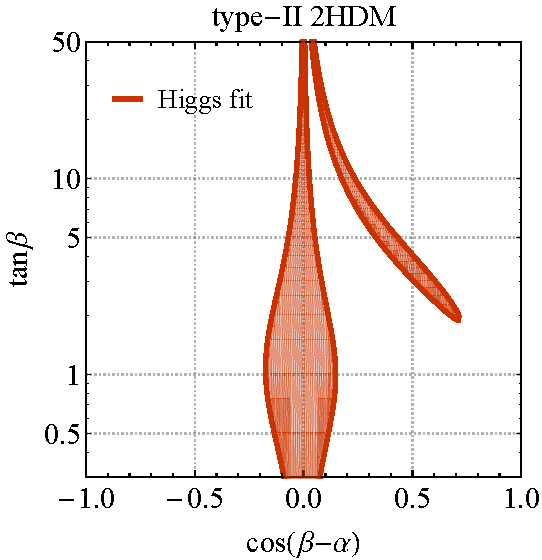
\includegraphics[width=0.435\textwidth]{texinputs/00_theory/figures/figure3l} \qquad 
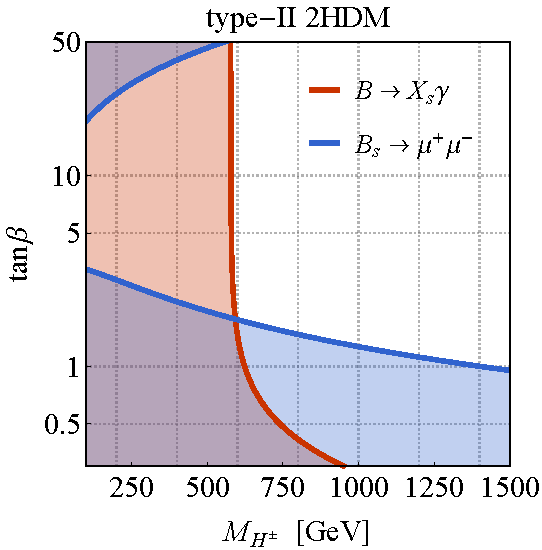
\includegraphics[width=0.45\textwidth]{texinputs/00_theory/figures/figure3r}
\vspace{4mm}
\caption{\label{fig:higgsflavourfit} Left: Parameter space allowed by a global fit to the LHC Run-I Higgs coupling strength measurements.  The lines show the contours which restrict the allowed parameter space at the 95\%~CL for a type-II 2HDM. Right: Parameter space in the $M_{H^\pm}\hspace{0.5mm}$--$\hspace{0.5mm}\tan \beta$ plane that is disfavoured by the flavour observables $B \to X_s \gamma$ (red) and $B_s \to \mu^+ \mu^-$ (blue). The uncoloured region in the upper right corner of the plot is allowed at 95\%~CL. }
\end{figure}

Indirect constraints on $\tan \beta$ as a function of $M_{H^\pm}$ arise from $B \to X_s \gamma$~\cite{Hermann:2012fc,Misiak:2015xwa,Misiak:2017bgg}, $B$-meson mixing~\cite{Abbott:1979dt,Geng:1988bq,Buras:1989ui,Kirk:2017juj} as well as  $B_s \to \mu^+ \mu^-$~\cite{Skiba:1992mg,Logan:2000iv,Chankowski:2000ng,Bobeth:2001sq,Bobeth:2013uxa,CMS:2014xfa,Aaij:2017vad}, but also follow from $Z \to b \bar b$~\cite{Denner:1991ie,Haisch:2007ia,Freitas:2012sy}. For the case of the type-II 2HDM, the most stringent constraints on the $M_{H^{\pm}}\hspace{0.5mm}$--$\hspace{0.5mm}\tan \beta$ plane are depicted in the right panel of Figure~\ref{fig:higgsflavourfit}. From the shown results it is evident that $B \to X_s \gamma$ provides a lower limit on the charged Higgs mass of $M_{H^\pm} > 580 \, {\rm GeV}$ that is practically independent of $\tan \beta$ for $\tan \beta \gtrsim 2$, while $B_s \to \mu^+ \mu^-$ is the leading constraint for very heavy charged Higgses, excluding for instance values of $\tan \beta < 1.3$ for $M_{H^\pm} = 1 \, {\rm TeV}$. As discussed in~\cite{Bauer:2017ota}, the constraints on $\tan \beta$ that follow from the existing LHC searches for heavy Higgses (see for instance~\cite{Aaboud:2017sjh,Sirunyan:2018zut,Aaboud:2017hnm,Aaboud:2018xuw})  are at the moment all weaker than the limits provided by flavour physics.  Since the  indirect constraints   arise from loop corrections they can in principle be weakened by the presence of additional particles that are too heavy to be produced at the LHC. We thus consider the bounds from flavour only as indicative, and will not directly impose them on the parameter space of the \hdma in what follows. 

%\subsection[Constraints on $\sin \theta$]{Constraints on $\bm{\sin theta}$}
\subsection*{Constraints on $\bm{\sin \theta}$}

EW precision measurements constrain the splittings between the masses $M_H, M_A, M_{H^\pm}$ and~$M_a$, since the exchange of spin-0 states modifies the propagators of the $W$- and $Z$-bosons at the one-loop level and beyond. For $M_H=M_{H^\pm}$ and $\cos(\beta-\alpha)=0$, these corrections vanish due to a custodial symmetry in the tree-level potential $V_H$~\cite{Haber:1992py,Pomarol:1993mu,Gerard:2007kn,Grzadkowski:2010dj,Haber:2010bw} introduced in~\eqref{eq:VH} and the masses of the CP-odd mass eigenstates can be treated as free parameters. This custodial symmetry is also present if $M_A=M_{H^\pm}$ and $\cos(\beta-\alpha)=0$, but the presence of the pseudoscalar mixing term in~\eqref{eq:VHP}  breaks this symmetry softly~\cite{Bauer:2017ota}. As a result, the pseudoscalar mixing angle $\theta$ and the mass splitting between $M_H$, $M_A$ and $M_a$ are constrained in such a case. An illustrative example of the resulting constraints is given in the left panel of Figure~\ref{fig:EWVAC}. To keep $\sin \theta$ and $M_a$ as free parameters, we consider below only \hdma model realisations in which the masses of the $H$, $A$ and $H^\pm$ are equal. Notice that the choice $M_H = M_A = M_{H^\pm}$ is also adopted  in some 2HDM interpretations of the searches for heavy spin-0 resonances performed at the LHC~(cf.~\cite{Aaboud:2017gsl,Aaboud:2017rel,Sirunyan:2018taj}~for example). 

%\subsection[Constraints on $M_a$]{Constraints on $\bm{M_a}$}
\subsection*{Constraints on $\bm{M_a}$}

Invisible decays of the Higgs boson allow to set a lower limit on the mass of  the~pseudoscalar~$a$ in \hdma scenarios with light DM~\cite{Bauer:2017ota}. In the case of $m_\chi = 1 \, {\rm GeV}$, it turns out for instance that mediator mass $M_a \lesssim 100 \, {\rm GeV}$ are excluded by imposing the 95\%~CL limit ${\rm BR} (h \to  \text{invisible}) \lesssim 25\%$~\cite{Aad:2015pla,Khachatryan:2016whc}. This limit is largely independent of the choices of the other parameters since ${\rm BR} (h \to  \text{invisible}) \simeq {\rm BR} (h \to a a^\ast \to 2 \chi 2 \bar \chi) \simeq 100\%$ for sufficiently light DM. To evade the limits from invisible Higgs decays, we consider in this whitepaper only $a$ masses larger than $100 \, {\rm GeV}$ when studying $\MET$ signatures at the LHC. 

%\subsection[Constraints on $\lambda_3$]{Constraints on $\bm{\lambda_3}$}
\subsection*{Constraints on $\bm{\lambda_3}$}

The requirement that the scalar potential~\eqref{eq:V2HDMa} of the \hdma  is bounded from below~(BFB), restricts the possible choices of the Higgs masses, mixing angles and quartic couplings. Assuming that $\lambda_{P1}, \lambda_{P2} > 0$, it is easy to see that the  BFB conditions in the~\hdma are identical to those found in the pure 2HDM~\cite{Gunion:2002zf}. For our choice $M_H = M_A = M_{H^\pm}$ of heavy Higgs masses, one finds that the tree-level BFB conditions can be cast into  two inequalities. The first inequality connects $\lambda_3$ with the cubic SM Higgs self-coupling $\lambda = M_h^2/(2 v^2) \simeq 0.13$ and simply reads   
\begin{align} \label{eq:BFB1}
\lambda_3 > 2 \lambda  \,.
\end{align}
The second BFB condition relates $\lambda_3$ with $\tan \beta$, $\sin \theta$, the common heavy Higgs mass $M_H$ and $M_a$ and turns out to be more complicated. In the limit $M_H \gg M_h, M_a$ it however takes a rather simple form that we quote here for illustration: 
\begin{align} \label{eq:BFB2}
\lambda_3 > \frac{M_H^2 -M_a^2}{v^2} \sin^2 \theta  - 2 \lambda \cot^2 (2 \beta )  \,.
\end{align}
This formula in essence  implies that large values of $M_H^2/v^2 \sin^2 \theta$ are only compatible with the requirements from BFB if the quartic coupling $\lambda_3$ is sufficiently large.  Notice that the interplay between BFB and perturbativity of $\lambda_3$,~i.e.~$\lambda_3 < 4 \pi$, leads to a non-decoupling of $H, A$ and $H^\pm$ for $|M_H - M_a| \neq 0$ and $\sin \theta  \neq 0$~\cite{Goncalves:2016iyg} such that the spin-0 states are potentially within LHC reach. The right plot in~Figure~\ref{fig:EWVAC} which shows the constraints in the $M_{a}\hspace{0.5mm}$--$\hspace{0.5mm} M_H$ plane that derive from the exact version of~\eqref{eq:BFB2} puts the latter statement on solid ground. From the figure one observes that for $\tan \beta = 1$, $\sin \theta = 0.35$ and $M_H = M_A = M_{H^\pm}$, values of $\lambda_3 \gtrsim 2$ are needed in order for $M_H \simeq 1 \, {\rm TeV}$ to be allowed by BFB.  Notice that due to the $\sin^2 \theta$ dependence in~\eqref{eq:BFB2}, close to non-perturbative couplings $\lambda_3 \gtrsim 8$ would be required to make $1 \, {\rm TeV}$ 2HDM Higgses viable for are larger pseudoscalar mixing angle of $\sin \theta = 0.7$. In order for heavy Higgs above $1 \, {\rm TeV}$ to be acceptable while keeping $\lambda_3$ perturbative, we will choose $\sin \theta = 0.35$ and $\lambda_3 = 3$ as our benchmark in this whitepaper.  

\begin{figure}
\centering
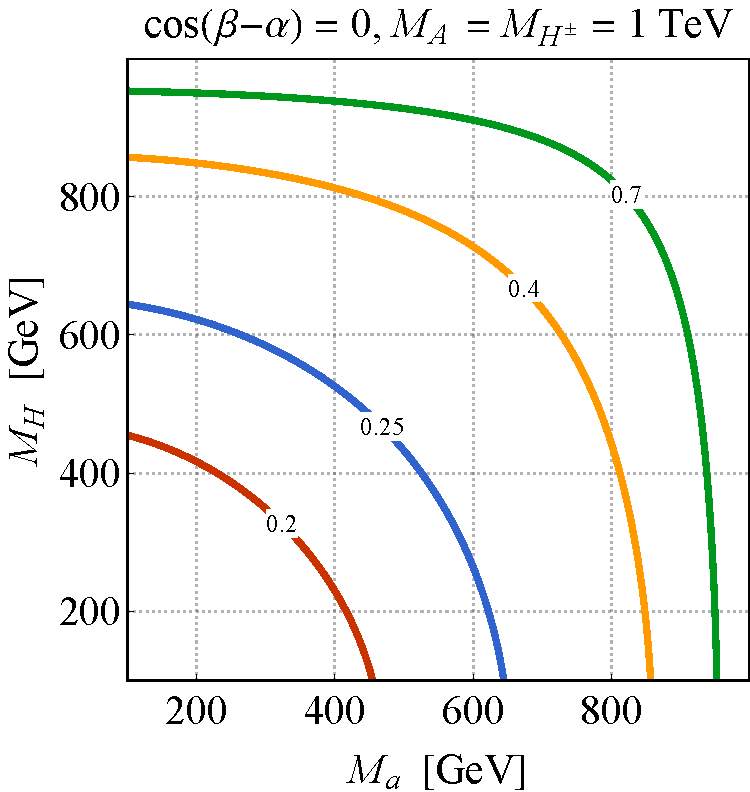
\includegraphics[height=.45\textwidth]{texinputs/00_theory/figures/figure4l} \qquad 
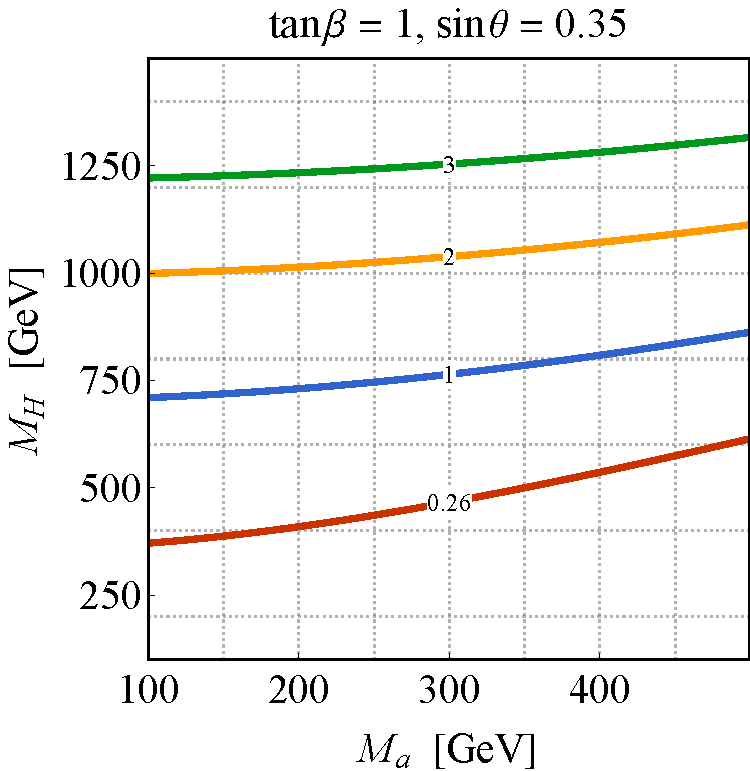
\includegraphics[height=.45\textwidth]{texinputs/00_theory/figures/figure4r}
\vspace{4mm}
\caption{\label{fig:EWVAC} Left: Values of $M_a$ and $M_H$ allowed by EW precision constraints assuming $\cos(\beta-\alpha)=0$, $M_A= M_{H^\pm}=1 \, {\rm TeV}$ and four different values of $\sin \theta$, as indicated by the contour labels.  The parameter space below and to the left of the contours is excluded. Right: Constraints in the $M_{a}\hspace{0.5mm}$--$\hspace{0.5mm} M_H$ plane following from the  requirements of having a  BFB \hdma scalar potential. The shown results correspond to $\tan \beta = 1$, $\sin \theta = 0.35$ and degenerate heavy Higgs masses $M_H = M_A = M_{H^\pm}$. The region above  each contour  is excluded for the indicated value of $\lambda_3$.}  
\end{figure}

%\subsection[Constraints on $\lambda_{P1}$ and $\lambda_{P2}$]{Constraints on  $\bm{\lambda_{P1}}$ and $\bm{\lambda_{P2}}$}
\subsection*{Constraints on $\bm{\lambda_{P1}}$ and $\bm{\lambda_{P2}}$}

The quartic couplings $\lambda_3$, $\lambda_{P1}$ and $\lambda_{P2}$ affect all  cubic Higgs interactions. In the case of the $Haa$ and $Aah$ couplings, one obtains under the assumption that  $\cos (\beta-\alpha) = 0$ and $M_H = M_A = M_{H^\pm}$, the following expressions~\cite{Bauer:2017ota}
\begin{eqnarray} \label{eq:cubic}
\begin{split}
g_{Haa}   & = \frac{1}{M_H v}  \Big [  \cot \left ( 2 \beta \right) \left (  2 M_h^2 - 2 \lambda_3 v^2 \right )  \sin^2 \theta + \sin \left ( 2 \beta \right ) \left (\lambda_{P1}-\lambda_{P2} \right ) v^2 \cos^2 \theta \Big  ] \,, \\[2mm]
g_{Aah}   & = \frac{1}{M_H v} \, \Big [ M_h^2  + M_H^2   -  M_a^2 - 2 \lambda_3 v^2 + 2 \left (  \lambda_{P1} \cos^2 \beta + \lambda_{P2} \sin^2 \beta  \right ) v^2 \Big ] \sin \theta \cos \theta \,. \hspace{6mm}
\end{split}
\end{eqnarray}
Because $\Gamma (H \to aa) \propto g_{Haa}^2$ and $\Gamma (A \to ah) \propto g_{Aah}^2$, the relations~\eqref{eq:cubic} imply  that  in order to keep the total widths $\Gamma_H$ and $\Gamma_A$ small, parameter choices of the form $\lambda_3 = \lambda_{P1} = \lambda_{P2}$ are well suited. 

\subsection*{Benchmark parameter choices}

The above discussion motivates the following choice of parameters
\begin{gather} 
 M_H  = M_A = M_{H^\pm} \,, \quad m_\chi = 10 \, {\rm GeV} \,,\notag  \\[1mm]
\cos (\beta - \alpha) = 0\,, \quad   \tan \beta = 1\,, \quad  \sin\theta = 0.35\,, \label{eq:benchmark} \\[1mm]
y_\chi  = 1\,, \quad \lambda_3 =  \lambda_{P1} = \lambda_{P2} =3 \,. \notag 
\end{gather}
In these  type-II \hdma  benchmark scenarios the only free parameters are then 
\begin{align}\label{eq:2hdmascan}
\big\{ M_H\,,\,\, M_a\big\} \,,
\end{align}
and the results of our $\MET$ sensitivity studies will always be presented in the corresponding two-dimensional parameter plane. 

We  emphasise that small departures from the  above parameter choices  will lead to a qualitatively  similar mono-$X$ phenomenology in the \hdma model. The signatures that are most sensitive to the mass splitting between the $H$ and the $A$, the parameter $\sin \theta$ and the quartic couplings $\lambda_{3}$, $\lambda_{P1}$, $\lambda_{P2}$ turn out to be  the mono-$Z$ and mono-Higgs channels. Four benchmark scenarios that illustrate these model dependences have been proposed and studied in~\cite{Bauer:2017ota}.  We believe that the specific benchmark  chosen in this whitepaper nicely exemplifying  the rich structure of $\MET$ signatures in the \hdma model, and the choices~\eqref{eq:benchmark} should therefore serve well as a starting point for further more detailed experimental and theoretical investigations.

As a final validation (or first application) of the proposed benchmark scenario, we present in  Figure~\ref{fig:Gammas} the predictions for the ratios $\Gamma_H/M_H$~(left) and $\Gamma_A/M_A$~(right). We see that the heavy neutral Higgs states $H$ and $A$ are relatively narrow even for values $M_H > 1 \, {\rm TeV}$ and $M_a = 100 \, {\rm GeV}$. The narrow width approximation~(NWA) is thus applicable in the entire parameter space considered in our $M_a\hspace{0.5mm}$--$\hspace{0.5mm}M_H$ scans. 

\begin{figure}
\centering
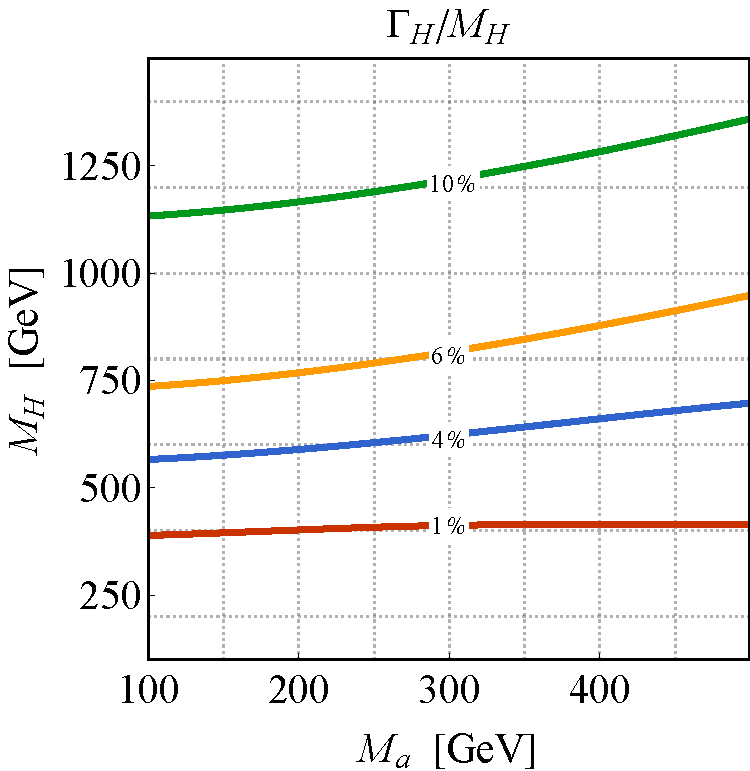
\includegraphics[height=.45\textwidth]{texinputs/00_theory/figures/figure5l} \qquad 
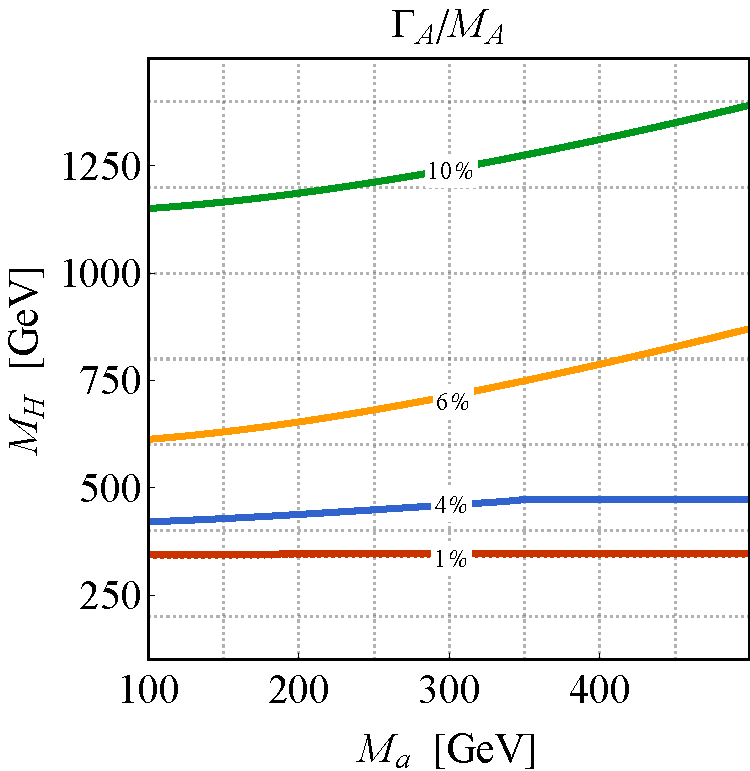
\includegraphics[height=.45\textwidth]{texinputs/00_theory/figures/figure5r}
\vspace{4mm}
\caption{\label{fig:Gammas}  Predictions for  $\Gamma_H/M_H$~(left panel) and $\Gamma_A/M_A$~(right panel). The shown results correspond to the type-II \hdma benchmark parameter choices given in~\eqref{eq:benchmark}.}
\end{figure}

\section{Comparison to other DM models}
\label{sec:comparison}

In this section we briefly discuss DM models that also feature a 2HDM sector. Our discussion will focus on the similarities and differences  between these scenarios and the \hdma model  for what concerns the mono-$X$ phenomenology. 

\subsection*{2HDM with an extra scalar singlet}

Instead of mixing an additional CP-odd singlet $P$ with the pseudoscalar $A$, as done in~\eqref{eq:VHP}, it is also possible to consider the mixing of a  scalar singlet~$S$ with  the CP-odd spin-0 states~$h,H$. Detailed studies of the direct-detection and relic-density phenomenology of this so-called 2HDM+s model have been presented in~\cite{Bell:2016ekl,Bell:2017rgi}.  Like in the case of the \hdma model, the presence of  non-SM Higgs bosons in the 2HDM+s model can lead to novel $\MET$ signatures that are not captured by a simplified DM model with just a single scalar mediator. In the pure alignment limit, the most interesting collider signals are mono-$Z$, mono-Higgs and the $t X + \MET$  channels, because  these signatures can all arise resonantly. Away from alignment, the scalar mediator couples to the EW gauge bosons and as a result it may also be possible to have a sizeable amount of $\MET$ in association with a $Z$ or $W$ boson or in  vector boson fusion (VBF). Notice that due to the CP properties of the $a$ the latter $\MET$ signatures are not present in the \hdma model. 

\subsection*{2HDM with doublet-singlet DM}

In both the \hdma and the 2HDM+s model the DM particle is  a EW singlet. The DM particle may however also be a mixture of a EW singlet and doublet(s)~\cite{Mahbubani:2005pt,Enberg:2007rp,Cohen:2011ec,Cheung:2013dua}, as in the minimal supersymmtric SM where it has both bino and higgsino components. Generically, this is referred to as singlet-doublet DM. The phenomenology of 2HDM models with singlet-doublet DM has been discussed in~\cite{Berlin:2015wwa,Arcadi:2018pfo}. In these works only the $b+\MET$ and $t \bar t+\MET$ signatures have been considered and found to provide only weak constraints. The recent study~\cite{Bauer:2017fsw} suggests that stronger constraints may  arise in the 2HDM with doublet-singlet DM from $Z + \MET$ and $tX+\MET$ searches. This feature warrants further investigations. 

\subsection*{2HDM with  higher-dimensional couplings to DM}

A gauge-invariant DM model where a pseudoscalar is embedded into a 2DHM that has renormalisable couplings to SM fields but an effective coupling to DM via the dimension-five operator $H_1^\dagger H_2 \bar \chi \gamma_5 \chi$ has been  discussed in~\cite{Bauer:2017fsw}. It has been shown that  such an  effective DM coupling can be obtained in different UV completions such as the \hdma model or  a 2HDM with doublet-singlet DM by integrating out heavy particles. Apart from the $t X+\MET$ signatures, the whole suit of mono-$X$ signals has been considered in~\cite{Bauer:2017fsw}. It was found that a resonant mono-$Z$ signal via $pp \to H \to AZ \to  Z + \chi \bar \chi$ is a universal prediction in all DM pseudoscalar mediator models, while other signatures such as mono-Higgs are model dependent. Given that a sizeable $H^\pm \to A W$ rate is also a generic feature of DM pseudoscalar models if $M_{H^\pm} > M_A + M_W$, channels like $tW+\MET$~\cite{Pani:2017qyd} should also  provide relevant constraints on the DM model introduced in~\cite{Bauer:2017fsw}. 

\subsection*{Inert doublet model}

In the scenarios discussed so far the DM particle has always been a fermion. The so-called inert doublet model~(IDM)~\cite{Deshpande:1977rw,Barbieri:2006dq,Cao:2007rm} is an intriguing DM model based on a 2HDM sector that can provide DM in the form of the spin-0 resonances $H, A$.  A $Z_2$ symmetry renders the DM candidate stable and also implies  that the bosonic states  that originate from the second~(dark) Higgs doublet can only be pair-produced. Since the dark scalars do not couple to the SM fermions, $H,A,H^\pm$ production arises in the IDM dominantly from Drell-Yan processes. The IDM offers a rich spectrum of LHC $\MET$ signatures that ranges from mono-jet, mono-$Z$, mono-$W$, mono-Higgs to  ${\rm VBF}+\MET$~\cite{Dolle:2009ft,Miao:2010rg,Gustafsson:2012aj,Belanger:2015kga,Ilnicka:2015jba,Poulose:2016lvz,Datta:2016nfz,Hashemi:2016wup,deFlorian:2016spz,Belyaev:2016lok,Dutta:2017lny}.  While the prospects to probe the IDM parameter space via the mono-jet channel seem to be limited~\cite{Belyaev:2016lok}, LHC searches for multiple leptons~\cite{Dolle:2009ft,Miao:2010rg,Gustafsson:2012aj,Belanger:2015kga,Datta:2016nfz,Hashemi:2016wup}, multiple jets~\cite{Poulose:2016lvz,Dutta:2017lny}  or a combination thereof~\cite{Hashemi:2016wup} are expected to allow to test the IDM in limits that are not accessible by direct detection of~DM or measurements of the invisible decay width of the SM Higgs. Furthermore, in scenarios in which the mass of DM is almost degenerate with~$M_{H^\pm}$, searches for disappearing charged tracks provide a rather unique handle on the IDM high-mass regime~\cite{Belyaev:2016lok}. Notice that while the IDM can lead to the same $\MET$ signals  than the \hdma model, the resulting kinematic distributions will in general not be the same, due to the different production mechanisms and decay topologies in the two models. Selection cuts that are optimised for a \hdma interpretation of a given mono-$X$ search will thus often not be ideal in the IDM context. Dedicated ATLAS and CMS  analyses of the mono-$X$ signatures in the IDM do unfortunately not exist at the moment. Such studies would however be highly desirable.

\subsection*{2HDM with an extra scalar mediator and scalar DM}

The DM scenario proposed in~\cite{vonBuddenbrock:2016rmr} contains like the 2HDM+s model an extra scalar singlet, which however does not couple to a fermionic DM current $\bar \chi \chi$ but to the scalar operator~$\chi^2$. The latter work focuses on the parameter space of the model where the mediator $s$ is dominantly produced via either  $pp \to H + j \to 2s + j \to j + 4 \chi$ or $pp \to H \to sh \to h + 2\chi$. The resulting mono-jet and mono-Higgs cross sections however turn out to be safely below the existing experimental limits. In case the mass hierarchy  $M_A > M_H + M_Z$ is realised, the channel $pp \to A \to HZ$ is also interesting, since it either leads to a mono-$Z$ or a $Zh+\MET$ signature, depending on whether $H \to 2 s \to 4 \chi$ or $H \to h s \to h \chi^2$ is the leading decay. We add that an effective version of the model brought forward in~\cite{vonBuddenbrock:2016rmr}  has already been constrained by ATLAS~\cite{Aaboud:2017uak} using the mono-Higgs channel. 







